\section{Máquina de Boltzmann}


\begin{frame}{Máquina de Boltzmann}%
  \justiying%
  Rede estocástica com $\omega_{ij} = \omega_{ji}$.
  \\~\\
  Possui dois tipos de unidades distintas: unidades \textbf{visíveis} e unidades \textbf{escondidas}.
  \\~\\
  \textbf{Visíveis}: ligadas ao meio externo; correspondentes as variáveis do problema.
  \\~\\
  \textbf{Escondidas}: não tem ligação do o meio externo; determinam a relação entre as variáveis do problema.
\end{frame}

\subsection{Esquema}
\begin{frame}{Arquitetura de BMs}%
  \begin{figure}[h]{}%
    \label{fig:bm-diagram}%
    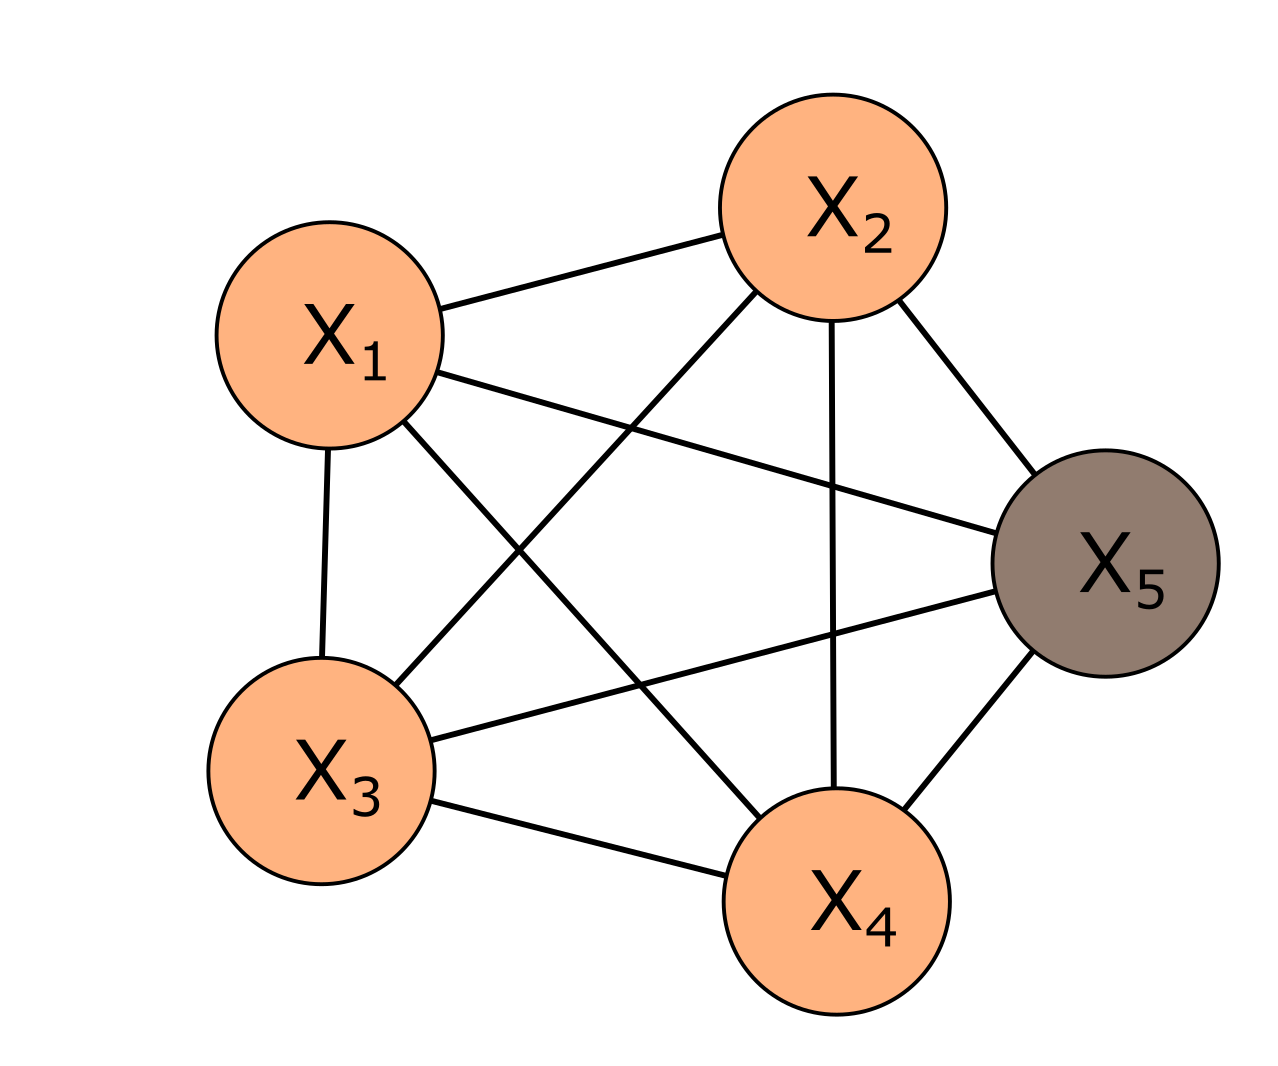
\includegraphics[scale=0.5]{images/bm_1.png}
    \caption{Diagrama de uma máquina de Boltzmann.\\
            \;}
  \end{figure}
\end{frame}

\begin{frame}{Arquitetura de BMs}%
  \begin{figure}[h]{}%
    \label{fig:bm-diagram}%
    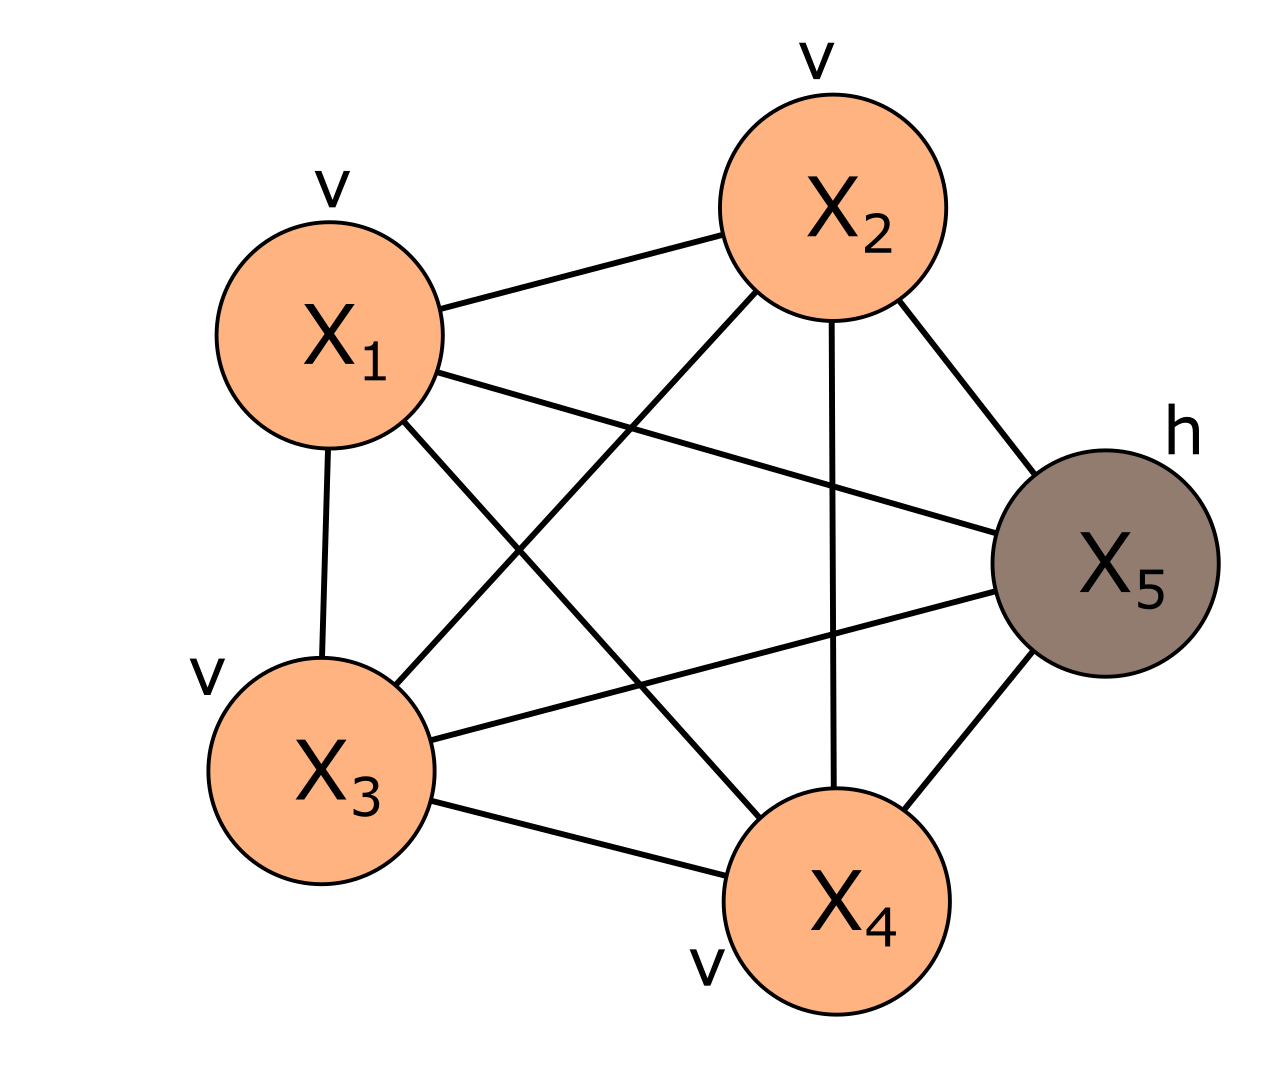
\includegraphics[scale=0.5]{images/bm_2.png}
    \caption{Diagrama de uma máquina de Boltzmann; unidades mais claras são as visíveis, e unidades mais escuras, as escondidas.}
  \end{figure}
\end{frame}

\subsection{Considerações}
\begin{frame}{O sistema}%
  \justifying%
  \onslide<1->{%
  Vamos considerar que temos uma rede com $N$ unidades visíveis, e $K$ unidades escondidas, }
  \onslide<2->{%
  em que as unidades visíveis estão no estado $v$, e as escondidas, no estado $h$.}
  \\~\\
  \onslide<3->{%
  Temos $2^{(N + K)}$ possibidades de estados em que a rede pode ser encontrada.
  }
  \\~\\
  \onslide<4->{%
  Uma unidade $\mathrm{x}_{i} = x_{i}$, sendo que $x_{i} \in \{0, 1\}$. 
  }
\end{frame}

\subsection{Aprendizagem}%
\begin{frame}{Objetivo da Máquina de Boltzmann}%
  \justiying%
  \onslide<1->{%
  Na máquina de Boltzmann fazemos o ajuste das conexões $\omega_{ij}$ para termos um certo estado nas unidades visíveis com uma distribuição de probabilidade desejada.
  \\~\\
  Se precisamos determinar as conexões $\omega_{ij}$, precisamos de um mecanismo para atualizar os pesos, temos que resolver:
  }
  \onslide<2->{%
  \begin{equation}%
    \label{eq:omega-learning}
    \omega^{(final)}_{ij} = \omega^{(inicial)}_{ij} + \Delta \omega_{ij}.
  \end{equation}
  }
  \\~\\
  \onslide<3->{%
  Lembrando que os pesos são ajustados baseados nos exemplos de treinamento que a rede recebe.  
  }

\end{frame}

\begin{frame}{Grandezas Importantes}%
  \justifying%
  Energia para rede com unidades visíveis no estado $v$, e escondidas, no estado $h$:
  \begin{equation}%
    \label{eq:bm-energy}
    H_{vh} = -\frac{1}{2} \sum_{i} \sum_{j} \omega_{ij} x_{i} x_{j} - \sum_{i} \phi_{i} x_{i}.
  \end{equation}
  \\~\\
  Podemos calcular a soma de todos os possíveis estados da rede pela função partição:
  \begin{equation}%
    \label{eq:bm-partition}
    Z = \sum_{u} \sum_{k} e^{(-\beta H_{uk})}.
  \end{equation}
\end{frame}

\begin{frame}{Grandezas Importantes}%
  A probabilidade $P_{v}$ de achar as unidades visíveis de uma máquina de Boltzmann em um determinado estado $v$, é
  \begin{equation}%
    \label{eq:bm-prob-marg}%
    P_{v} = \sum_{h} \frac{1}{Z} e^{-\beta H_{vh}}
  \end{equation}
\end{frame}

\begin{frame}{Entropia Relativa - Divergência Kullback-Leibler}%
  \justifying%
  Se temos duas distribuições de probabilidade distintas, por exemplo, $P$ e $R$, sobre um mesmo espaço de estados, podemos calcular a diferença entre estas distribuições pela entropia relativa, $E$, (ou divergência de Kullback-Leibler, $D_{KL}(R||P)$.
%  \begin{equation}%
%    \label{eq:dkl}
%    E = \sum_{v} R \ln \left[\frac{R}{P} \right]
%  \end{equation}
\end{frame}
  
\begin{frame}{Entropia Relativa - Divergência Kullback-Leibler}%
  \justifying%
  Com as máquinas de Boltzmann queremos determinar a probabilidade $P_{v}$ de achar as unidades visíveis em determinado estado $v$, como mostra a equação~(\ref{eq:bm-prob-marg}). Porém para este estado temos uma probabilidade deseja $R_{v}$.
  \begin{equation}%
    \label{eq:bm-entropy}
    E = \sum_{v} R_{v} \ln \left[\frac{R_{v}}{P_{v}} \right]
  \end{equation}
\end{frame}

\begin{frame}{Atualização de $\Delta \omega_{ij}$}%
  \justifying%
  Usamos a nossa entropia relativa como função custo.
  \\~\\
  Pelo método do grandiente descendente, podemos calcular $\Delta \omega_{ij}$,
  \begin{equation}%
    \label{eq:omega-delta}
    \Delta \omega_{ij} = -\eta \frac{\partial E}{\partial \omega_{ij}}.
  \end{equation}
  \\~\\
  $E$ é função de $P_{v}$.
  $P_{v}$ é função dos pesos $\omega_{ij}$.
\end{frame} 

\begin{frame}{Atualização de $\Delta \omega_{ij}$}%
  \justifying%
  Por simplificação, vamos considerar que a função de energia para a rede no estado $v$ e $h$ é dada apenas pela correlação entre as unidades (primeiro termo da equação~(\ref{eq:bm-energy})).
\end{frame}

\subsection{next one $\dots$}

\begin{frame}{frame teste}
%  Suponhamos que queremos, que temos um problema onde queremos saber descrever a distribuição de probabilidade com que certos eventos acontecem.
%  
%  a partir de um conjunto de treinamento, determinar a distribuição de probabilidade de encontrar os estados mais estáveis da rede
\end{frame}
